\section{Specific Requirements}
\subsection{External Interface Requirements}
    \subsubsection{User Interfaces}
    This application that we have should be able to receive information about each land and then track the progress of the farmers. We assume that each farmer signs up to our application and then inserts the data of the land, also we receive the forecasts of the meteorological data of Telangana. In these applications, farmers can create discussions and also ask about their problems. Policymakers can observe the farmland and choose the best and worst. There are notifications for farmers about the humidity, the amount of water that the land used, the forecast for weather in the app that helps them to improve their performance. You can see the mock up of our application in the following:
    
    \begin{figure}[H]
  \centering
  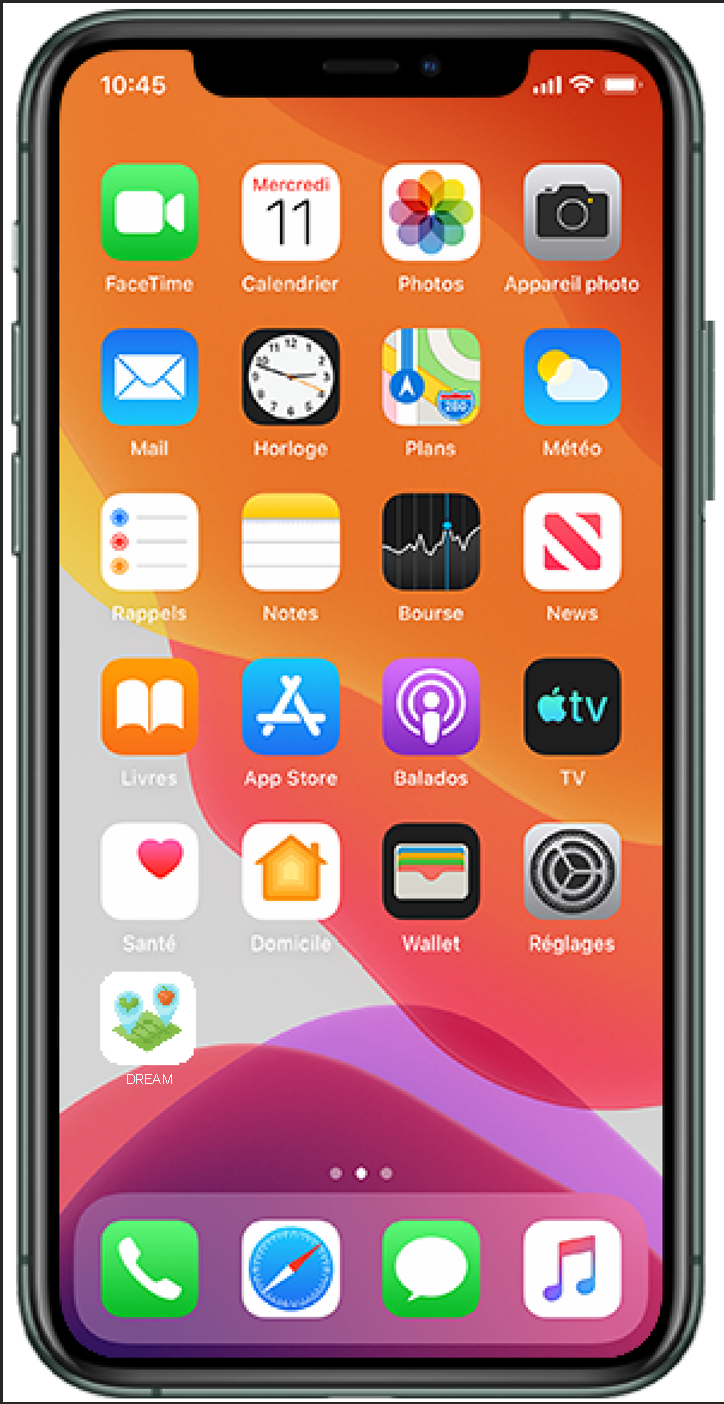
\includegraphics[width=0.5\textwidth,keepaspectratio]{figures/homescreen.png}
  \caption{App Icon}
\end{figure}
\begin{figure}[H]
  \centering
  \subfloat[Opening page] {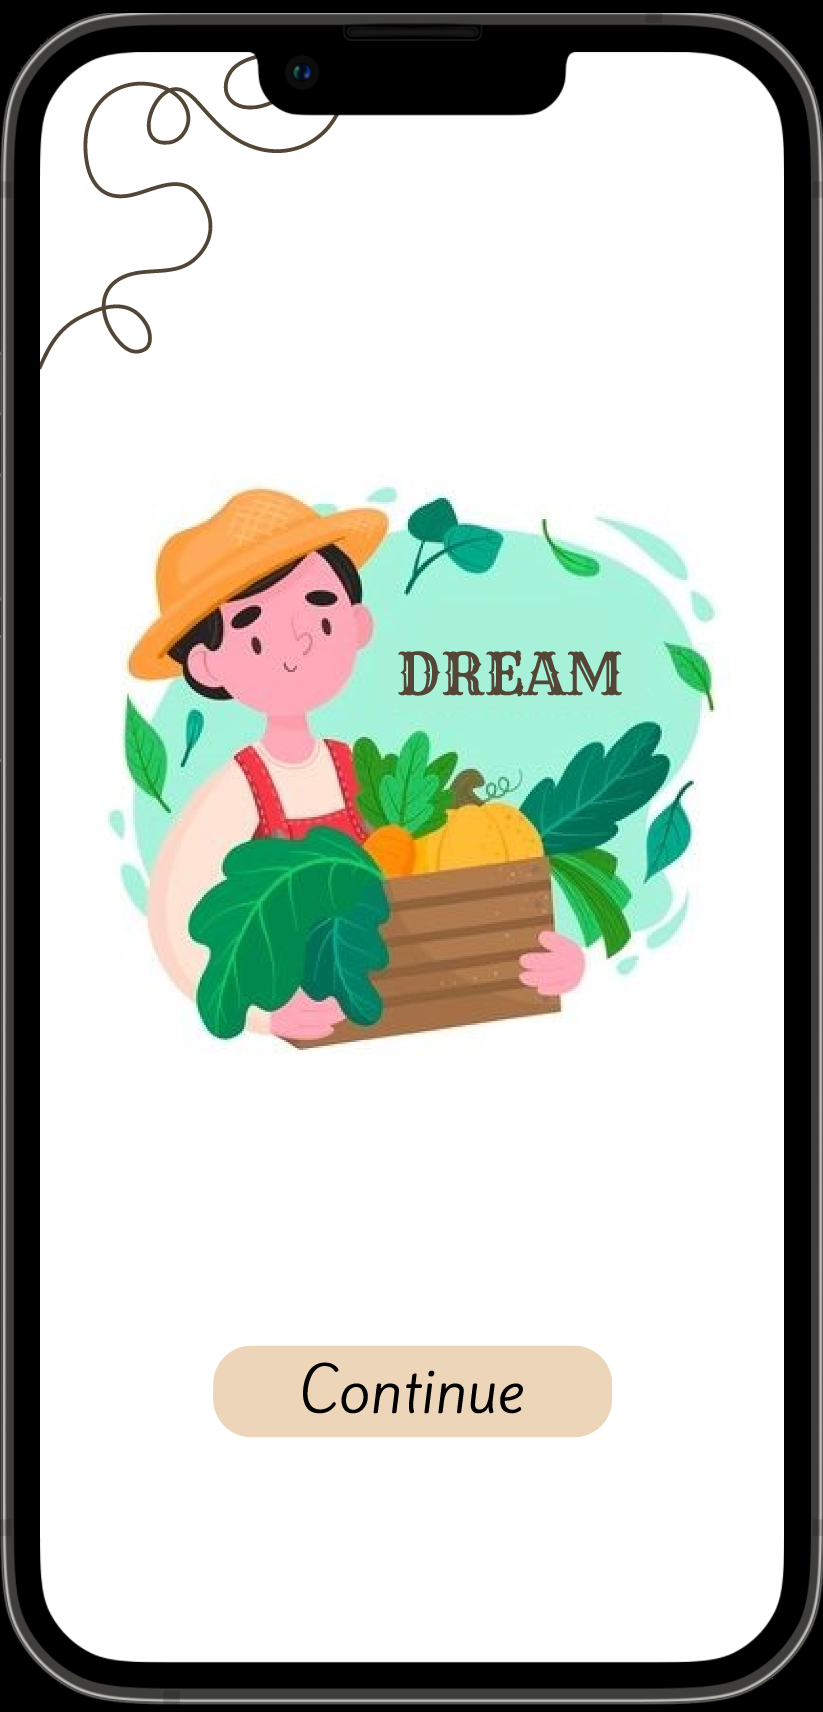
\includegraphics[width=0.4\textwidth,keepaspectratio]{figures/openning page.png}}
  \hfill
  \subfloat[sign in Farmers] {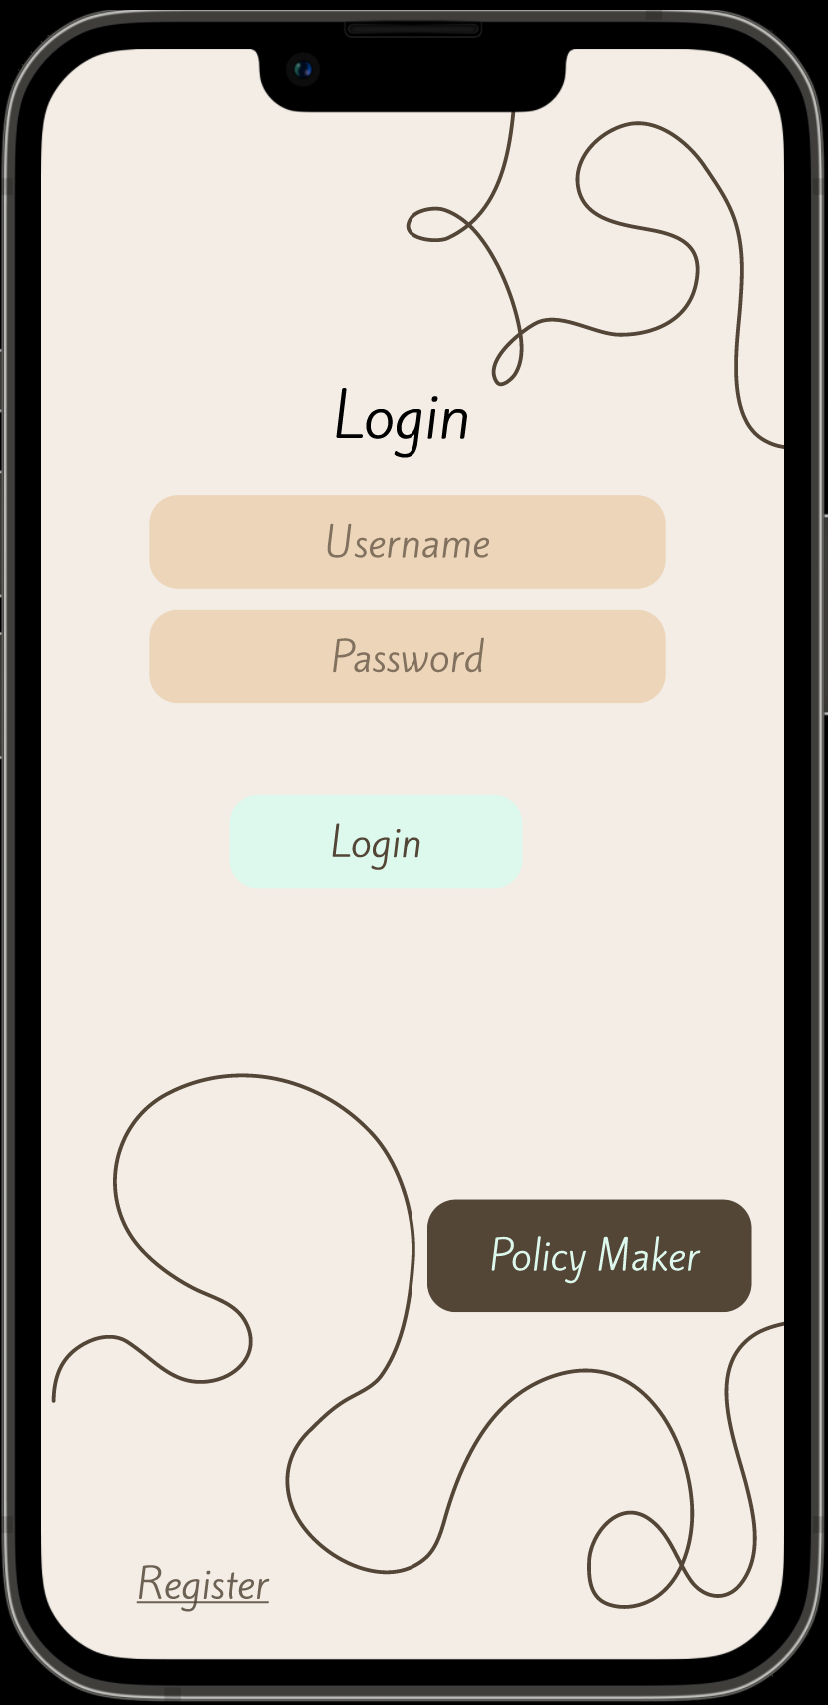
\includegraphics[width=0.4\textwidth,keepaspectratio]{figures/Loginpage.png}}
  \hfill
  \subfloat[sign in policy makers] {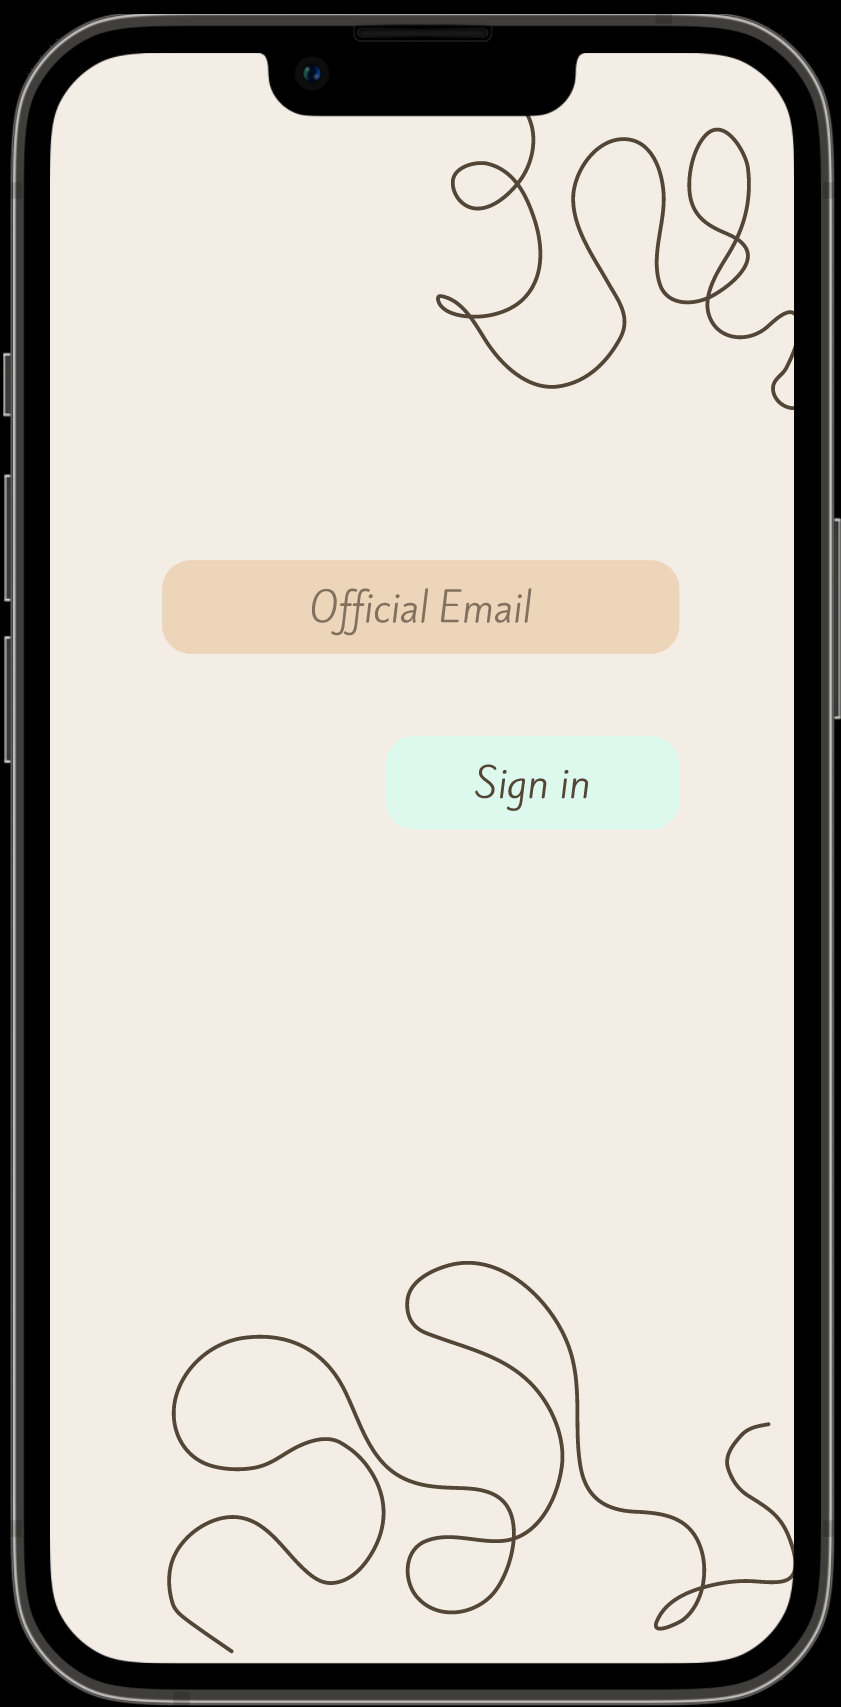
\includegraphics[width=0.4\textwidth,keepaspectratio]{figures/PolicymakerLogin.png}}
  \hfill
  \subfloat[sign up Farmers] {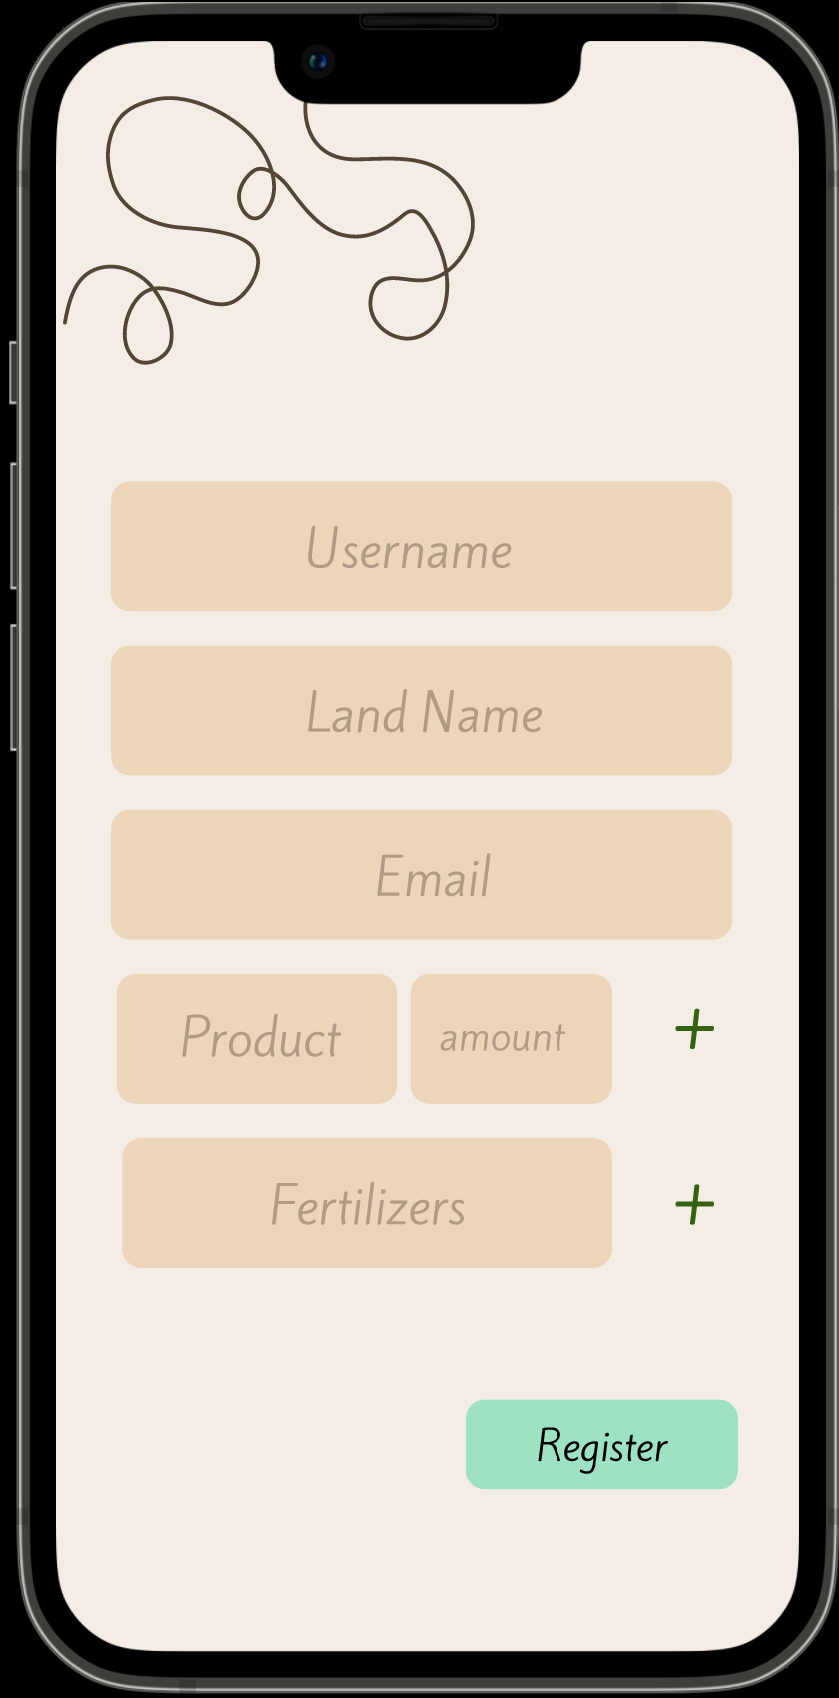
\includegraphics[width=0.4\textwidth,keepaspectratio]{figures/signupFarmers.png}}
  \hfill

  %\caption{Mockup}
\end{figure}
\begin{figure}[H]
  \centering
  
  \subfloat[Farmers Main page] {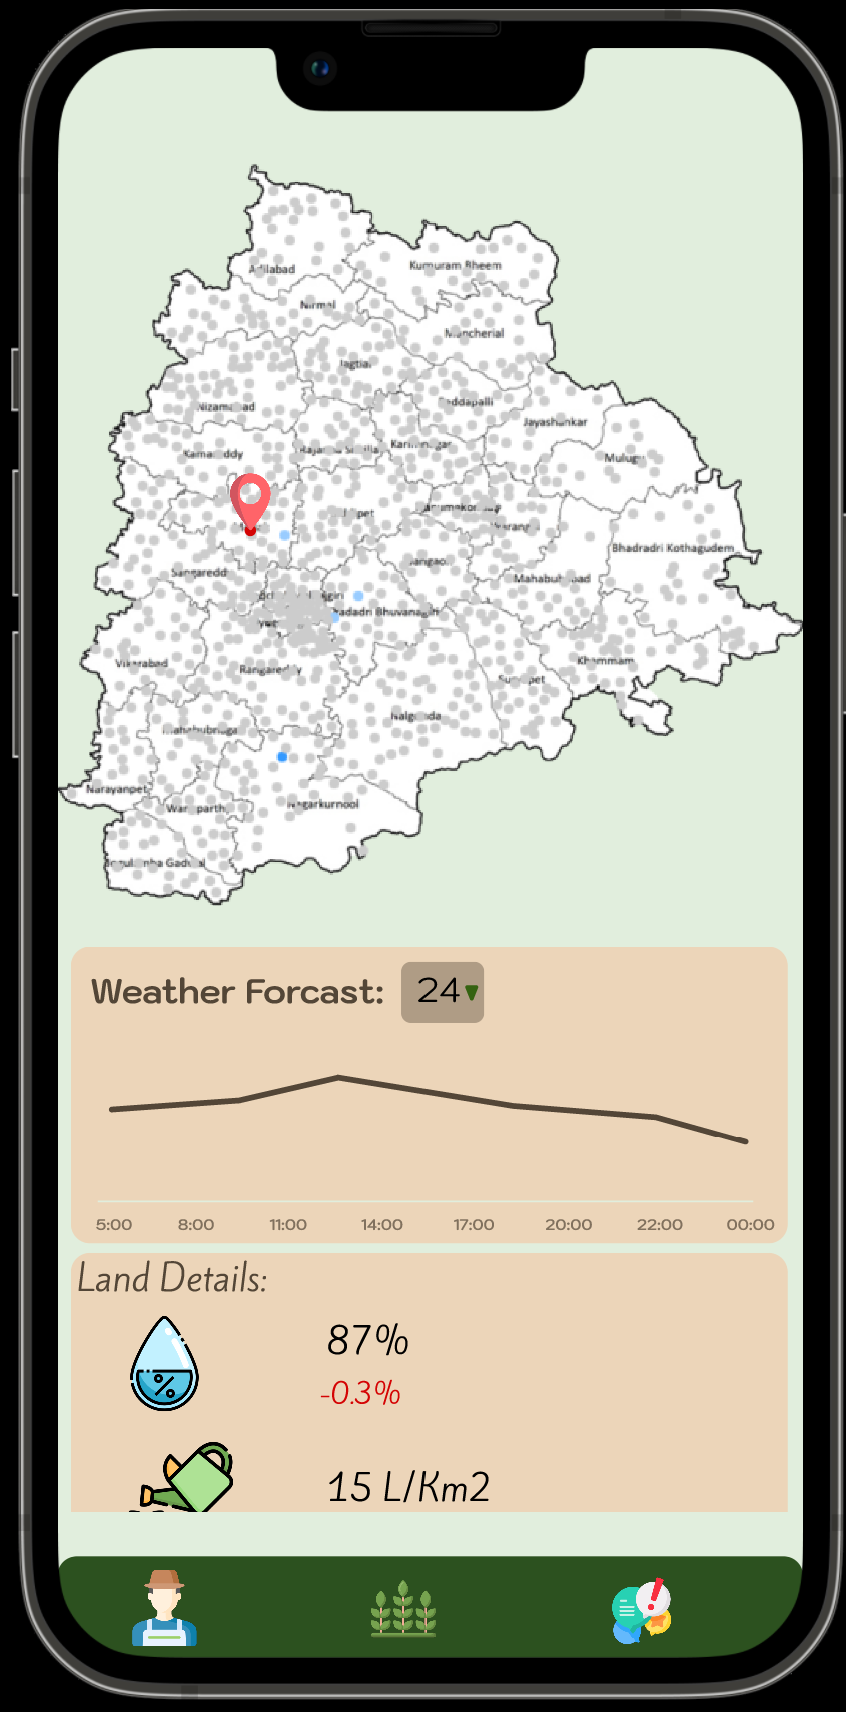
\includegraphics[width=0.4\textwidth,keepaspectratio]{figures/FarmersMainPage.png}}
  \hfill
  \hfill
  \subfloat[Policy-Makers Main page] {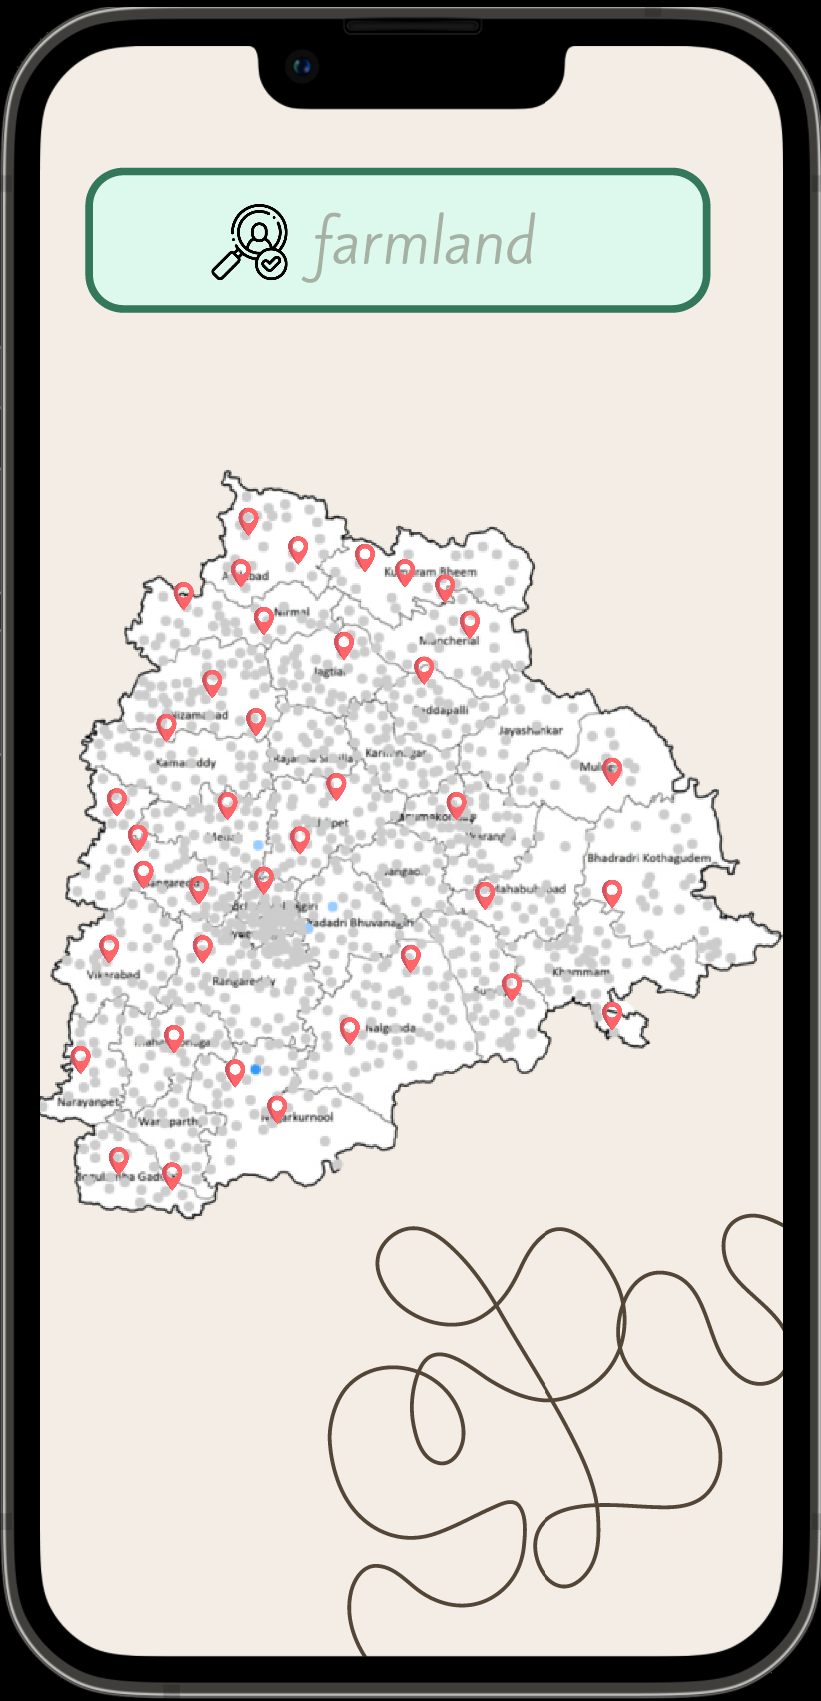
\includegraphics[width=0.4\textwidth,keepaspectratio]{figures/policyMakerMainPage.png}}
  \hfill

  \caption{Mockup}
\end{figure}

    \subsubsection{Hardware Interfaces}
    In this system, farmers need to have a smartphone with GPS or a desktop computer that they can, register and add their land to the application and track the changes and also their suggestions. Also, their smartphone should contain a touch screen or keyboard which helps them to start a discussion in the application, ask their questions and share their experiences. The policymaker should also have a smartphone or a desktop computer that login into their account and observe the farmer’s progress in the system. As we just have a mobile application for this program yet, they just need a smartphone.
    \subsubsection{Software Interfaces}
    Our system contains the following interfaces:\\
    Telangana’s map, We’ll use some API that allows us to
\begin{itemize}
    \item Locate the farmlands
    \item Getting information from water irrigation systems
    \item Getting data related to each land from sensors
    \item Getting meteorological information from Telangana’s government
\end{itemize}
The application should receive information about each land and update the data of each profile in real-time.\\
Also, we need push notification services when:
\begin{itemize}
    \item some urgent information change in the servers 
    \item they receive a message from policymakers
    \item someone sends a message in the discussion that they start or join.
\end{itemize}.

    \subsubsection{Communication Interfaces}
    The devices connect to DREAM via an internet connection.
\clearpage
\subsection{Functional Requirements}
    \subsubsection{List of Requirements}
    \begin{longtable}{ !\Vline c !\Vline p{0.9\linewidth} !\Vline}
    \hline
    \textbf{R1} & Farmers certified with an authentication\\
    \textbf{R2} & Policy-Makers certified with an authentication\\
    \textbf{R3} & Policy-Makers should register to the application with extra mandatory fields\\
    \textbf{R4} & Only Policy-Makers can observe all the farm land\\
    \textbf{R5} & Only Policy-Makers can best and worst farmers\\
    \textbf{R6} & Policy-Makers can choose farmers who received special incentives\\
    \textbf{R7} & Policy-Makers must identify those farmers who need to be helped\\
    \textbf{R8} & Farmers can be asked to provide useful best practices to the others\\
    \textbf{R9} & Farmers must accept the GPS location for the application\\
    \textbf{R10} & Farmers must insert their product to the system\\
    \textbf{R11} & Farmers can visualize data relevant to them\\
    \textbf{R12} & Farmers must insert the fertilizers that they are using to the system\\
    \textbf{R13} & Farmers could see the list of forecast related to their location\\
    \textbf{R14} & Farmers can insert any problem they face \\
    \textbf{R15} & Farmers can start a discussion \\
    \textbf{R16} & Farmers can request for help and suggestions by other farmers \\
    \textbf{R17} & Farmers can join to an existing discussion \\
    \textbf{R18} & Farmers can terminate their own discussion \\
    \textbf{R19} & The system should receive the data related to meteorological short-term and long-term forecasts from Telengana's governments \\
    \textbf{R20} & The system should suggest fertilizer based on the farmers locations and products \\
    \textbf{R21} & The system should receive the data from sensors periodically \\
    \textbf{R22} & The system should receive data from water irrigation system periodically\\
    \textbf{R23} & The system should send notifications about the farm land to the farmers\\
    \textbf{R24} & The system sends a notification to farmers if they receive new message\\
    \textbf{R25} & The system sends a notification to farmers if the humidity if water decrease\\
    \textbf{R26} & The system sends a notification to farmers if policymakers choose them as worst or best farmers\\
    \hline
\end{longtable}

\clearpage
    \subsubsection{Mapping}
    \arrayrulecolor{tableBorderColor}
\setlength\arrayrulewidth{1pt}
\rowcolors{2}{white}{tableHighlightColor}
\setlength\LTleft{0pt}
\begin{longtable}{ !\Vline c !\Vline p{0.3\linewidth} !\Vline p{0.6\linewidth} !\Vline}
    \hline
    \multicolumn{1}{|c|}{\textbf{Goal}} & \multicolumn{1}{c|}{\textbf{Domain assumption}} & \multicolumn{1}{c|}{\textbf{Requirements}}\\
    G1 & D1,D4,D5,D13 & R1,R9,R10, R12,R13,R19,R21,R22\\
    G2 & D4,D5 & R2,R3,R4, R10,R21,R22\\
    G3 & D1,D4,D5,D7,D8,D10 & R2,R3,R4,R6,R10,R21,R22,R26\\
    G4 & D1,D4,D5,D7,D8 & R2,R3,R4,R7,R10,R21,R22,R26\\
    
    G5 & D1,D2,D11 & R1,R15,R16,R17, R24\\
    G6 & D1,D2,D11 & R1,R17, R18\\
    G7 & D1,D9,D11,D13 & R1,R15,R17,R24\\
    G8 & D1, D9 & R1,R15,R17,R18\\
    G9 & D1,D2,D11 & R1,R16,R18\\
    G10 & D9,D11 & R1,R14\\
    G11 & D1,D9,D11,D13 & R1,R9,R17,R18, R24\\
    G12 & D1,D4,D13 & R8, R10,R23,R25\\
    
    \hline
\end{longtable}

\arrayrulecolor{tableBorderColor}
\setlength\arrayrulewidth{1pt}
\rowcolors{2}{white}{white}
\setlength\LTleft{0pt}
\begin{longtable}{ !\Vline c !\Vline p{0.9\linewidth} !\Vline}
    \hline
    \cellcolor{tableHighlightColor} \textbf{G1} & Allow farmers to see the details of their farm lands\\ \hline
     \cellcolor{purpleHiglight} \textbf{D1} & every farmer has at least one land\\ \hline
       \cellcolor{purpleHiglight} \textbf{D4} & farmers insert all of the information about production correctly\\ \hline
        \cellcolor{purpleHiglight} \textbf{D5} & farmer insert all of the information correctly\\ \hline
          \cellcolor{purpleHiglight} \textbf{D13} &  each user has a smartphone \\ \hline
    \cellcolor{pinkHighlight} \textbf{R1} & Farmers certified with an authentication\\
    \hline
    \cellcolor{pinkHighlight} \textbf{R9} & Farmers must accept the GPS location for the application\\
    \hline
    \cellcolor{pinkHighlight} \textbf{R10} & Farmers must insert their product to the system\\
    \hline
    \cellcolor{pinkHighlight} \textbf{R12} & Farmers must insert the fertilizers that they are using to the system\\
    \hline
    \cellcolor{pinkHighlight} \textbf{R13} & Farmers could see the list of forecast related to their location\\
    \hline
    \cellcolor{pinkHighlight} \textbf{R19} & The system should receive the data related to meteorological short-term and long-term forecasts from Telengana's governments\\
    \hline
    \cellcolor{pinkHighlight} \textbf{R21} & The system should suggest fertilizer based on the farmers locations and products\\
    \hline
    \cellcolor{pinkHighlight} \textbf{R22} & The system should receive data from water irrigation system periodically\\
    \hline
    \cellcolor{tableHighlightColor} \textbf{G2} & Allow policy makers to see the details of different lands\\ \hline
       \cellcolor{purpleHiglight} \textbf{D4} & farmers insert all of the information about production correctly\\ \hline
        \cellcolor{purpleHiglight} \textbf{D5} & farmer insert all of the information correctly\\ 
        \hline
    \cellcolor{pinkHighlight} \textbf{R2} & Policy-Makers certified with an authentication\\
    \hline
    \cellcolor{pinkHighlight} \textbf{R3} & Policy-Makers should register to the application with extra mandatory fields\\
    \hline
    \cellcolor{pinkHighlight} \textbf{R4} & Only Policy-Makers can observe all the farm land\\
    \hline
    \cellcolor{pinkHighlight} \textbf{R10} & Farmers must insert their product to the system\\
    \hline
    \cellcolor{pinkHighlight} \textbf{R21} & The system should receive the data from sensors periodically\\
    \hline
    \cellcolor{pinkHighlight} \textbf{R22} & The system should receive data from water irrigation system periodically\\
    \hline
    \cellcolor{tableHighlightColor} \textbf{G3} & Allow policy makers to identify farmers who are performing well\\ \hline
     \cellcolor{purpleHiglight} \textbf{D1} & every farmer has at least one land\\ \hline
       \cellcolor{purpleHiglight} \textbf{D4} & farmers insert all of the information about production correctly\\ \hline
        \cellcolor{purpleHiglight} \textbf{D5} & farmer insert all of the information correctly\\ \hline
          \cellcolor{purpleHiglight} \textbf{D7} &  amount of used water report correctly by irrigation system \\ \hline
          \cellcolor{purpleHiglight} \textbf{D8} &  policy maker asses the former based on true information \\ \hline
          \cellcolor{purpleHiglight} \textbf{D10} &  amount of reported humidity is correctly \\ \hline
    \cellcolor{pinkHighlight} \textbf{R2} & Policy-Makers certified with an authentication\\
    \hline
    \cellcolor{pinkHighlight} \textbf{R3} & Policy-Makers should register to the application with extra mandatory fields\\
    \hline
    \cellcolor{pinkHighlight} \textbf{R4} & Only Policy-Makers can observe all the farm land\\
    \hline
    \cellcolor{pinkHighlight} \textbf{R6} & policy-Makers can choose farmers who received special incentives\\
    \hline
    \cellcolor{pinkHighlight} \textbf{R10} & Farmers must insert their product to the system\\
    \hline
    \cellcolor{pinkHighlight} \textbf{R21} & The system should receive the data from sensors periodically\\
    \hline
    \cellcolor{pinkHighlight} \textbf{R22} & The system should receive data from water irrigation system periodically\\
    \hline
    \cellcolor{pinkHighlight} \textbf{R26} & The system sends a notification to farmers if policymakers choose them as worst or best farmers\\
    \hline
    \cellcolor{tableHighlightColor} \textbf{G4} & Allow policy makers to identify farmers who need help\\ \hline
    \cellcolor{purpleHiglight} \textbf{D1} & every farmer has at least one land\\ \hline
       \cellcolor{purpleHiglight} \textbf{D4} & farmers insert all of the information about production correctly\\ \hline
        \cellcolor{purpleHiglight} \textbf{D5} & farmer insert all of the information correctly\\ \hline
          \cellcolor{purpleHiglight} \textbf{D7} &  amount of used water report correctly by irrigation system \\ \hline
          \cellcolor{purpleHiglight} \textbf{D8} &  policy maker asses the former based on true information \\ \hline
    \cellcolor{pinkHighlight} \textbf{R2} & Policy-Makers certified with an authentication\\
    \hline
    \cellcolor{pinkHighlight} \textbf{R3} & Policy-Makers should register to the application with extra mandatory fields\\
    \hline
    \cellcolor{pinkHighlight} \textbf{R4} & Only Policy-Makers can observe all the farm land\\
    \hline
    \cellcolor{pinkHighlight} \textbf{R7} & Policy-Makers must identify those farmers who need to be helped\\
    \hline
    \cellcolor{pinkHighlight} \textbf{R10} & Farmers must insert their product to the system\\
    \hline
    \cellcolor{pinkHighlight} \textbf{R21} & The system should receive the data from sensors periodically\\
    \hline
    \cellcolor{pinkHighlight} \textbf{R22} & The system should receive data from water irrigation system periodically\\
    \hline
    \cellcolor{pinkHighlight} \textbf{R26} & The system sends a notification to farmers if policymakers choose them as worst or best farmers\\
    \hline
    \cellcolor{tableHighlightColor} \textbf{G5} & Allow farmers to create new forum\\ \hline
     \cellcolor{purpleHiglight} \textbf{D1} & The internet works properly\\ \hline
      \cellcolor{purpleHiglight} \textbf{D2} &  Its better for users to have smartphones\\ \hline
      \cellcolor{purpleHiglight} \textbf{D11} &  farmers insert problems about farm land,production\\ \hline
    \cellcolor{pinkHighlight} \textbf{R1} & Users certified with an authentication\\
    \hline
    \cellcolor{pinkHighlight} \textbf{R15} & Farmers can start a discussion\\
    \hline
    \cellcolor{pinkHighlight} \textbf{R16} & Farmers can request for help and suggestions by other farmers\\
    \hline
    \cellcolor{pinkHighlight} \textbf{R17} & Farmers can join to an existing discussion\\
    \hline
    \cellcolor{pinkHighlight} \textbf{R24} & The system sends a notification to farmers if they receive new message\\
    \hline
    \cellcolor{tableHighlightColor} \textbf{G6} & Allow farmers to join in discussions\\ \hline
     \cellcolor{purpleHiglight} \textbf{D1} & The internet works properly\\ \hline
      \cellcolor{purpleHiglight} \textbf{D2} &  Its better for users to have smartphones\\ \hline
      \cellcolor{purpleHiglight} \textbf{D11} &  farmers insert problems about farm land,production\\ \hline
      \cellcolor{pinkHighlight} \textbf{R1} & Farmers certified with an authentication\\
    \hline
    \cellcolor{pinkHighlight} \textbf{R17} & Farmers can join to an existing discussion\\
    \hline
    \cellcolor{pinkHighlight} \textbf{R18} &  Farmers can terminate their own discussion\\
    \hline
    \cellcolor{tableHighlightColor} \textbf{G7} &  Allow farmers to send message in discussions\\ \hline
     \cellcolor{purpleHiglight} \textbf{D1} & The internet works properly\\ \hline
     \cellcolor{purpleHiglight} \textbf{D9} & just authenticated farmer can send message to forum\\ \hline
       \cellcolor{purpleHiglight} \textbf{D11} & farmers insert problems about farm land,production\\ \hline
       
      \cellcolor{purpleHiglight} \textbf{D13} &  each user has a smartphone\\ \hline
    \cellcolor{pinkHighlight} \textbf{R1} & Farmers certified with an authentication\\
    \hline
    \cellcolor{pinkHighlight} \textbf{R15} & Farmers can start a discussion\\
    \hline
    \cellcolor{pinkHighlight} \textbf{R17} & Farmers can join to an existing discussion\\
    \hline
    \cellcolor{pinkHighlight} \textbf{R24} & The system sends a notification to farmers if they receive new message\\
    \hline
    
    \cellcolor{tableHighlightColor} \textbf{G8} & Allow farmers to create new forum\\ \hline
    \cellcolor{purpleHiglight} \textbf{D1} & The internet works properly\\ \hline
     \cellcolor{purpleHiglight} \textbf{D9} & just authenticated farmer can send message to forum\\ \hline
    \cellcolor{pinkHighlight} \textbf{R1} & Farmers certified with an authentication\\
    \hline
    \cellcolor{pinkHighlight} \textbf{R15} & Farmers can start a discussion\\
    \hline
    \cellcolor{pinkHighlight} \textbf{R17} & Farmers can join to an existing discussion\\
    \hline
    \cellcolor{pinkHighlight} \textbf{R18} &  Farmers can terminate their own discussion\\
    \hline
    \cellcolor{tableHighlightColor} \textbf{G9} & Allow farmers to leave in discussions\\ \hline
     \cellcolor{purpleHiglight} \textbf{D1} & The internet works properly\\ \hline
      \cellcolor{purpleHiglight} \textbf{D2} &  Its better for users to have smartphones\\ \hline
      \cellcolor{purpleHiglight} \textbf{D11} &  farmers insert problems about farm land,production\\ \hline
      \cellcolor{purpleHiglight} \textbf{D11} &  farmers insert problems about farm land,production\\ \hline
      \cellcolor{pinkHighlight} \textbf{R1} & Farmers certified with an authentication\\
    \hline
    \cellcolor{pinkHighlight} \textbf{R16} & Farmers can leave a discussion\\
    \hline
    \cellcolor{pinkHighlight} \textbf{R18} &  Farmers can terminate their own discussion\\
    \hline
    \cellcolor{tableHighlightColor} \textbf{G10} & Allow farmers to ask problems\\ \hline
      \cellcolor{purpleHiglight} \textbf{D9} & just authenticated farmer can send message to forum\\ \hline
      \cellcolor{purpleHiglight} \textbf{D11} & farmers insert problems about farm land,production\\ \hline
    \cellcolor{pinkHighlight} \textbf{R1} & Farmers certified with an authentication\\
    \hline
    \cellcolor{pinkHighlight} \textbf{R14} & Farmers can insert any problem they face \\
    \hline
    \cellcolor{tableHighlightColor} \textbf{G11} & Allow farmers to answer to problems\\ \hline
     \cellcolor{purpleHiglight} \textbf{D1} & The internet works properly\\ \hline
     \cellcolor{purpleHiglight} \textbf{D9} & just authenticated farmer can send message to forum\\ \hline
       \cellcolor{purpleHiglight} \textbf{D11} & farmers insert problems about farm land,production\\ \hline
      \cellcolor{purpleHiglight} \textbf{D13} &  each user has a smartphone\\ \hline
    \cellcolor{pinkHighlight} \textbf{R1} & Farmers certified with an authentication\\
    \hline
    \cellcolor{pinkHighlight} \textbf{R15} & Farmers can start a discussion\\
    \hline
    \cellcolor{pinkHighlight} \textbf{R17} & Farmers can join to an existing discussion\\
    \hline
    \cellcolor{pinkHighlight} \textbf{R18} &  Farmers can terminate their own discussion\\
    \hline
    \cellcolor{pinkHighlight} \textbf{R24} & The system sends a notification to farmers if they receive new message\\ \hline
    \cellcolor{tableHighlightColor} \textbf{G12} & Show farmers some personal suggestion\\ \hline
     \cellcolor{purpleHiglight} \textbf{D1} & every farmer has at least one land\\ \hline
      \cellcolor{purpleHiglight} \textbf{D4} & farmers insert all of the information about production correctly\\ \hline
      \cellcolor{purpleHiglight} \textbf{D13} & each user has a smartphone\\ \hline
    \cellcolor{pinkHighlight} \textbf{R8} & Farmers can be asked to provide useful best practices to the others\\
    \hline
    \cellcolor{pinkHighlight} \textbf{R10} & Farmers must insert their product to the system\\
    \hline
    \cellcolor{pinkHighlight} \textbf{R23} & The system should send notifications about the farm land to the farmers\\
    \hline
    \cellcolor{pinkHighlight} \textbf{R25} & The system sends a notification to farmers if the humidity if water decrease\\
    \hline
    
\end{longtable}
    \subsubsection{Use Cases}
    
    \paragraph{Use Cases Description}\hfill
\begin{table}[H]
%\centering
\begin{tabular}{|l|l|}
\hline
\normalsize	
\textbf{Name} & Sign up\\\hline
\textbf{Actor} & farmer\\\hline
\textbf{Entry conditions} & Use the user has installed the application on her/his device\\\hline
\textbf{Event flow}  &  1. Click on "Sign Up" button"\\ 
&2. Fill all the mandatory fields and provide the necessary information\\
&3. Click on "Confirm" button\\
&4.the system saves the data \\\hline
\textbf{Exit conditions} & The user successfully registered and now he's able to use the application. \\\hline
\textbf{Exceptions }& 
1.the user is already signed up \\&
2.the user didn't fill all of the mandatory fields with valid data\\&
3.The username is already taken\\&
4.the e-mail is already registered\\&
5.All the exception are handled by notifying the user and taking\\& him back to the sign up activity
\\\hline
\end{tabular}
%\caption{\label{tab:widgets}An example table.}
\end{table}




\begin{table}[H]
%\centering
\begin{tabular}{|l|l|}
\hline
\normalsize	
\textbf{Name} & log in\\\hline
\textbf{Actor} & farmer\\\hline
\textbf{Entry conditions} & The user is previously successfully signed up 
\\&and has the application installed in his/her device\\\hline
\textbf{Event flow}  &  1. The user opens the application on his/device\\&
2. He enters his credentials in the “Username” and “Password” fields of\\&
the home page of “DREAM”\\&
3. The user clicks on the “Log in” button\\&
4. The user is successfully logged in his/her “DREAM”\\&
the system automatically redirects him/her to the home page\\\hline
\textbf{Exit conditions} & The user is successfully redirected to the home page \\\hline
\textbf{Exceptions }& 
1. The user enters an invalid Username\\&
2. The user enters invalid Password\\&
3. All the exceptions are handled by notifying the user and taking\\&
him/her back to the login activity\\&
\\\hline
\end{tabular}
%\caption{\label{tab:widgets}An example table.}
\end{table}


\begin{table}[H]
%\centering
\begin{tabular}{|l|l|}
\hline
\normalsize	
\textbf{Name} & insert the initial information \\\hline
\textbf{Actor} & farmer\\\hline
\textbf{Entry conditions}& The user has already logged in\\\hline
\textbf{Event flow} &1. The farmer select the farm land location\\&
2. He enters his credentials in the “Username” ,“land name” ,"email"\\& 
,"product","amount"and"fertilizer"\\&
3. the user click on  the register button\\&
4. The user is successfully logged in his/her “DREAM”\\&
the system automatically redirects him/her to the home page\\\hline
\textbf{Exit conditions} & The user is successfully redirected to the home page \\\hline
\textbf{Exceptions }& 
1. The user enters an empty Username field\\&
2. The user enters an empty land name field\\&
3. The user enters an empty Email field\\&
4. the user enter empty product \& amount field\\\hline
\end{tabular}
%\caption{\label{tab:widgets}An example table.}
\end{table}




\begin{table}[H]
%\centering
\begin{tabular}{|l|l|}
\hline
\normalsize	
\textbf{Name} & analyse  the initial conditions\\\hline
\textbf{Actor} & farmer\\\hline
\textbf{Entry conditions} & The farmer insert completely initial information and report \\\hline
\textbf{Event flow}  &  1.The system get initial information\\&
2. It get weather forecast based on GPS and land location \\&
3. system analyze the information \\\hline
\textbf{Exit conditions} & make personalized suggestion \\\hline
\textbf{Exceptions }& 
1. the forecast data is not accurate or invalid \\&
2. input data has conflict\\&
3. All the exceptions are handled by notifying the user and taking\\&
him/her back to the insert information page\\&
\\\hline
\end{tabular}
%\caption{\label{tab:widgets}An example table.}
\end{table}


\begin{table}[H]
%\centering
\begin{tabular}{|l|l|}
\hline
\normalsize	
\textbf{Name} & make personalized suggestion\\\hline
\textbf{Actor} & farmer\\\hline
\textbf{Entry conditions} & analysing of initial information has completed\\\hline
\textbf{Event flow}  &  1. get the analysing of initial information \\ 
&2. apply the ML/AL algorithm find best crop and fertilizer\\
&3. show the result to farmer \\
\textbf{Exit conditions} & The user successfully registered and now he's able to use the application. \\\hline
\textbf{Exceptions }& 
1.the user is already signed up \\&
2.the user didn't fill all of the mandatory fields with valid data\\&
3.The username is already taken\\&
4.the e-mail is already registered\\&
5.All the exception are handled by notifying the user and taking\\& him back to the sign up activity
\\\hline
\end{tabular}
%\caption{\label{tab:widgets}An example table.}
\end{table}

\begin{table}[H]
%\centering
\begin{tabular}{|l|l|}
\hline
\normalsize	
\textbf{Name} & Measure used water\\\hline
\textbf{Actor} & Irrigation system\\\hline
\textbf{Entry conditions} & Install irrigation system on the land\\\hline
\textbf{Event flow}  &  1.The irrigation system measure used water in specific frequency-time\\\hline
\textbf{Exit conditions} & Send measured data to access point \\\hline
\textbf{Exceptions}& 
1. Measured used water is not possible \\&
2. Irrigation system doesn't work correctly\\&
3. All the exceptions are handled by sent notification to access point 
\\\hline
\end{tabular}
%\caption{\label{tab:widgets}An example table.}
\end{table}


\begin{table}[H]
%\centering
\begin{tabular}{|l|l|}
\hline
\normalsize	
\textbf{Name} & Measure soil humidity\\\hline
\textbf{Actor} & Sensor\\\hline
\textbf{Entry conditions} & Install sensor with the specific distance in depth of soil\\\hline
\textbf{Event flow} & 1.the installed sensors sense humidity \\\hline
\textbf{Exit conditions} & Send measured data to access point \\\hline
\textbf{Exceptions}& 
1. Measured used soil humidity is not possible \\&
2. Sensors doesn't work correctly\\&
3. All the exceptions are handled by sent notification to access point 
\\\hline
\end{tabular}
%\caption{\label{tab:widgets}An example table.}
\end{table}



\begin{table}[H]
%\centering
\begin{tabular}{|l|l|}
\hline
\normalsize	
\textbf{Name} & send collected data to the  access point\\\hline
\textbf{Actor} & system\\\hline
\textbf{Entry conditions} & measure soil humidity  OR  measure used water OR  report forecast weather \\\hline
\textbf{Event flow}  &  1. get the measured soil humidity from sensors\\&
OR get measured used water from irrigation system \\&
OR get weather forecast from meteorological station \\&
2. collect information and prepare it to analyse\\\hline
\textbf{Exit conditions} & analyse the collected info \\\hline
\textbf{Exceptions }& 
1.The network doesn't work correctly  \\&
2.Sensors doesn't work correctly \\&
3.Irrigation systems doesn't work correctly \\&
4.Weather forecast doesn't report information correctly\\&
5.All the exceptions are handled by sent notification to access point
\\\hline
\end{tabular}
%\caption{\label{tab:widgets}An example table.}
\end{table}



\begin{table}[H]
%\centering
\begin{tabular}{|l|l|}
\hline
\normalsize	
\textbf{Name} & report forecast weather t\\\hline
\textbf{Actor} & Meteorological station\\\hline
\textbf{Entry conditions} & Meteorological station connects to the internet and GPS \\\hline
\textbf{Event flow} & 1.connect to the meteorological satellite \\&
2. get the weather forecast\\&
3.get the location information by GPS\\\hline
\textbf{Exit conditions} & send collected data to the access point \\\hline
\textbf{Exceptions }& 
1.The network doesn't work correctly  \\&
2.GPS doesn't work correctly \\&
3. Meteorological station devices work correctly\\&
5.All the exceptions are handled by sent notification to access point
\\\hline
\end{tabular}
%\caption{\label{tab:widgets}An example table.}
\end{table}

\begin{table}[H]
%\centering
\begin{tabular}{|l|l|}
\hline
\normalsize	
\textbf{Name} & evaluate farmer performance\\\hline
\textbf{Actor} & policy maker\\\hline
\textbf{Entry conditions} & analyse the collected info   \\\hline
\textbf{Event flow} & 1.get analysing collected environment data \\&
2. identify good and bad farmer based on analysed data\\\hline
\textbf{Exit conditions} & after identifying the high and  low performance farmer  \\\hline
\textbf{Exceptions }& 
1.analysed data is not accrued\\&
2.analysed data  has a shortage information \\&
3.analysed data is not reliable and semantic meaning  \\&
5.All the exceptions are handled by sent notification to access point
\\\hline
\end{tabular}
%\caption{\label{tab:widgets}An example table.}
\end{table}

\begin{table}[H]
%\centering
\begin{tabular}{|l|l|}
\hline
\normalsize	
\textbf{Name} & visualize the analysed information \\\hline
\textbf{Actor} & farmer\\\hline
\textbf{Entry conditions} &  analyse the collected info  \\\hline
\textbf{Event flow} & 1.get analysed data \\&
2. apply the specific algorithm to visualized the data\\&
\\\hline
\textbf{Exit conditions} & result is ready to show to farmer  \\\hline
\textbf{Exceptions }& 
1. analyzed data doesn't have enough quality to analyzed that can be visualized \\&
2.data doesn't have semantic meaning 
\\\hline
\end{tabular}
%\caption{\label{tab:widgets}An example table.}
\end{table}

\paragraph{Use Cases Diagram}\hfill
           

\begin{figure}[H]
%\centering
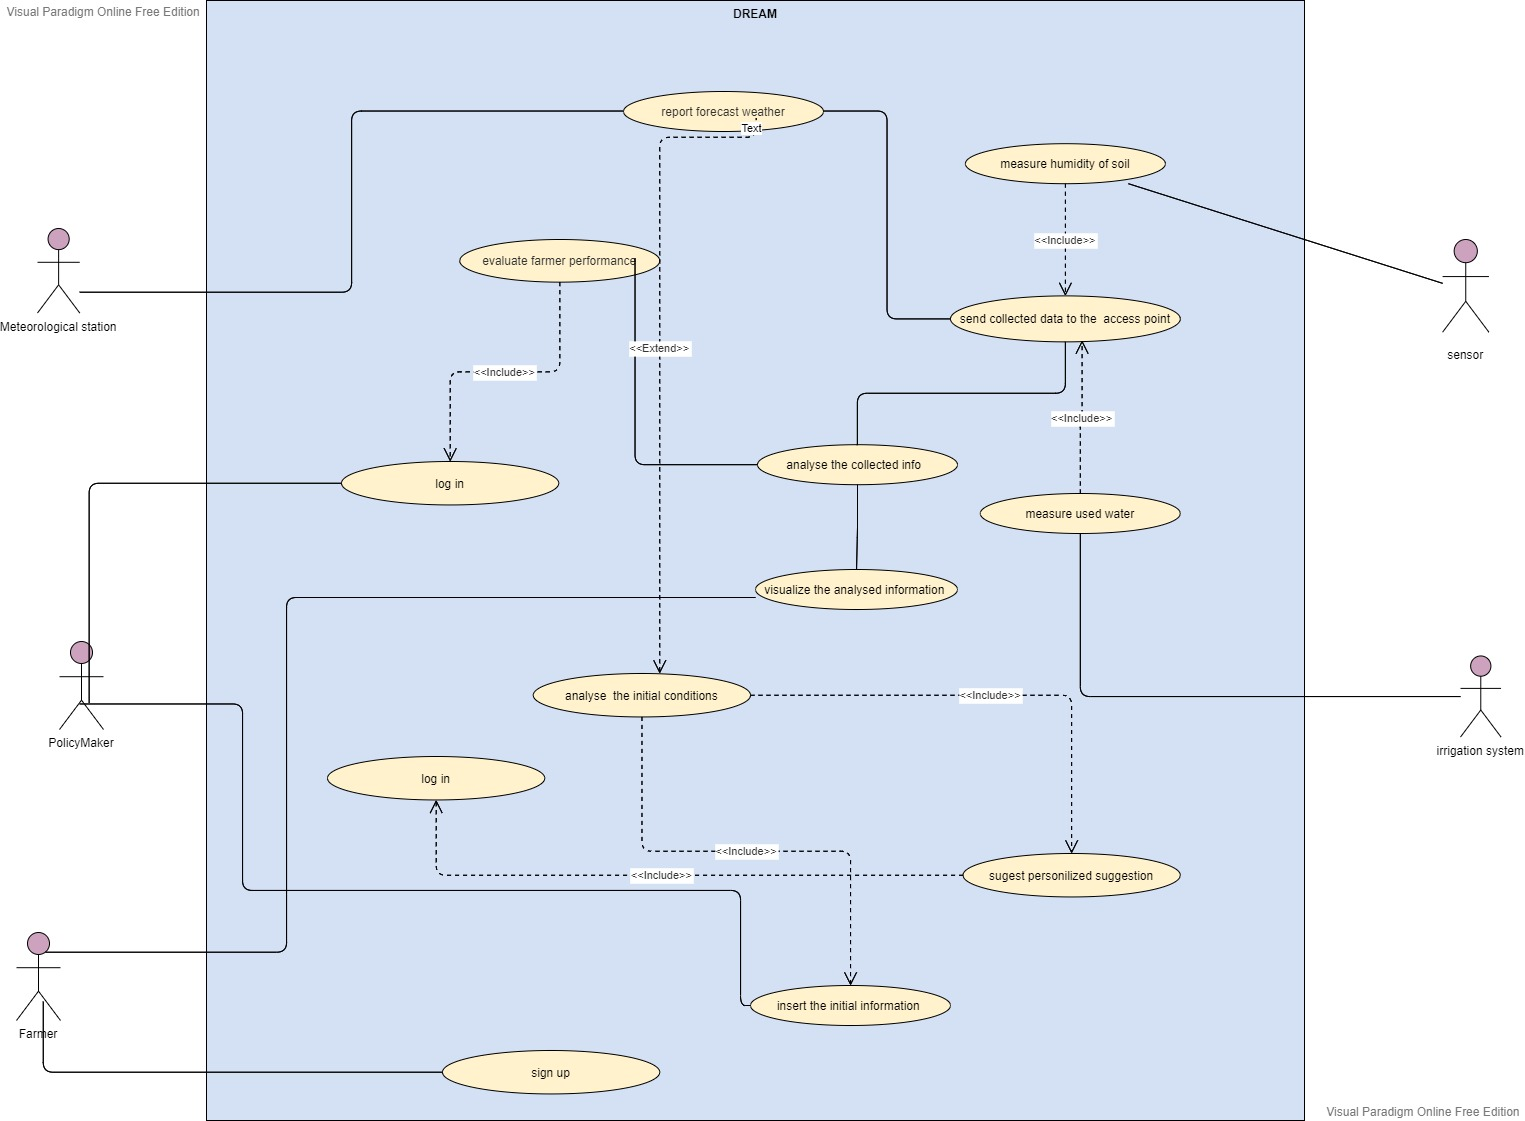
\includegraphics[width=1\textwidth]{figures/usecase.jpg}
%\caption{\label{fig:student } State Diagram 3 - evaluate the farmer by policymaker }
\end{figure}
       \subsubsection{Sequence diagram}
    \begin{figure}[H]
%\centering
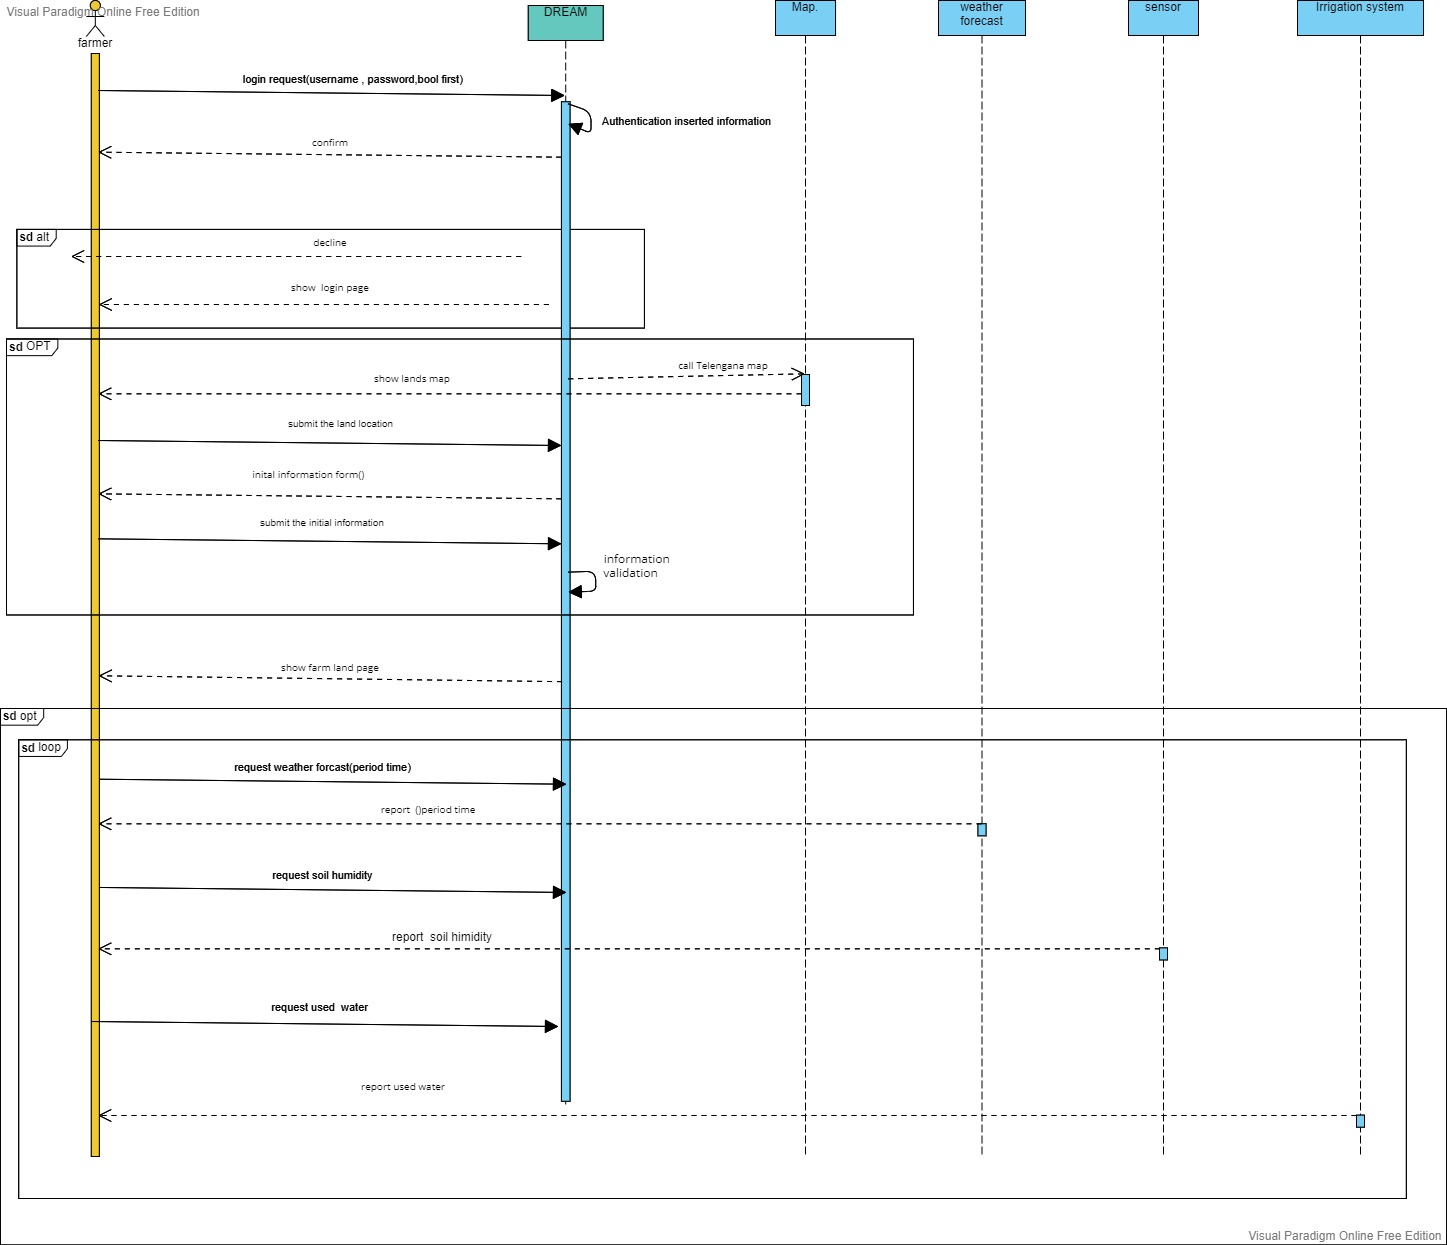
\includegraphics[width=1\textwidth]{figures/firstSequenceDiagram.jpg}
%\caption{\label{fig:student } State Diagram 3 - evaluate the farmer by policymaker }
\end{figure}
\begin{figure}[H]
%\centering
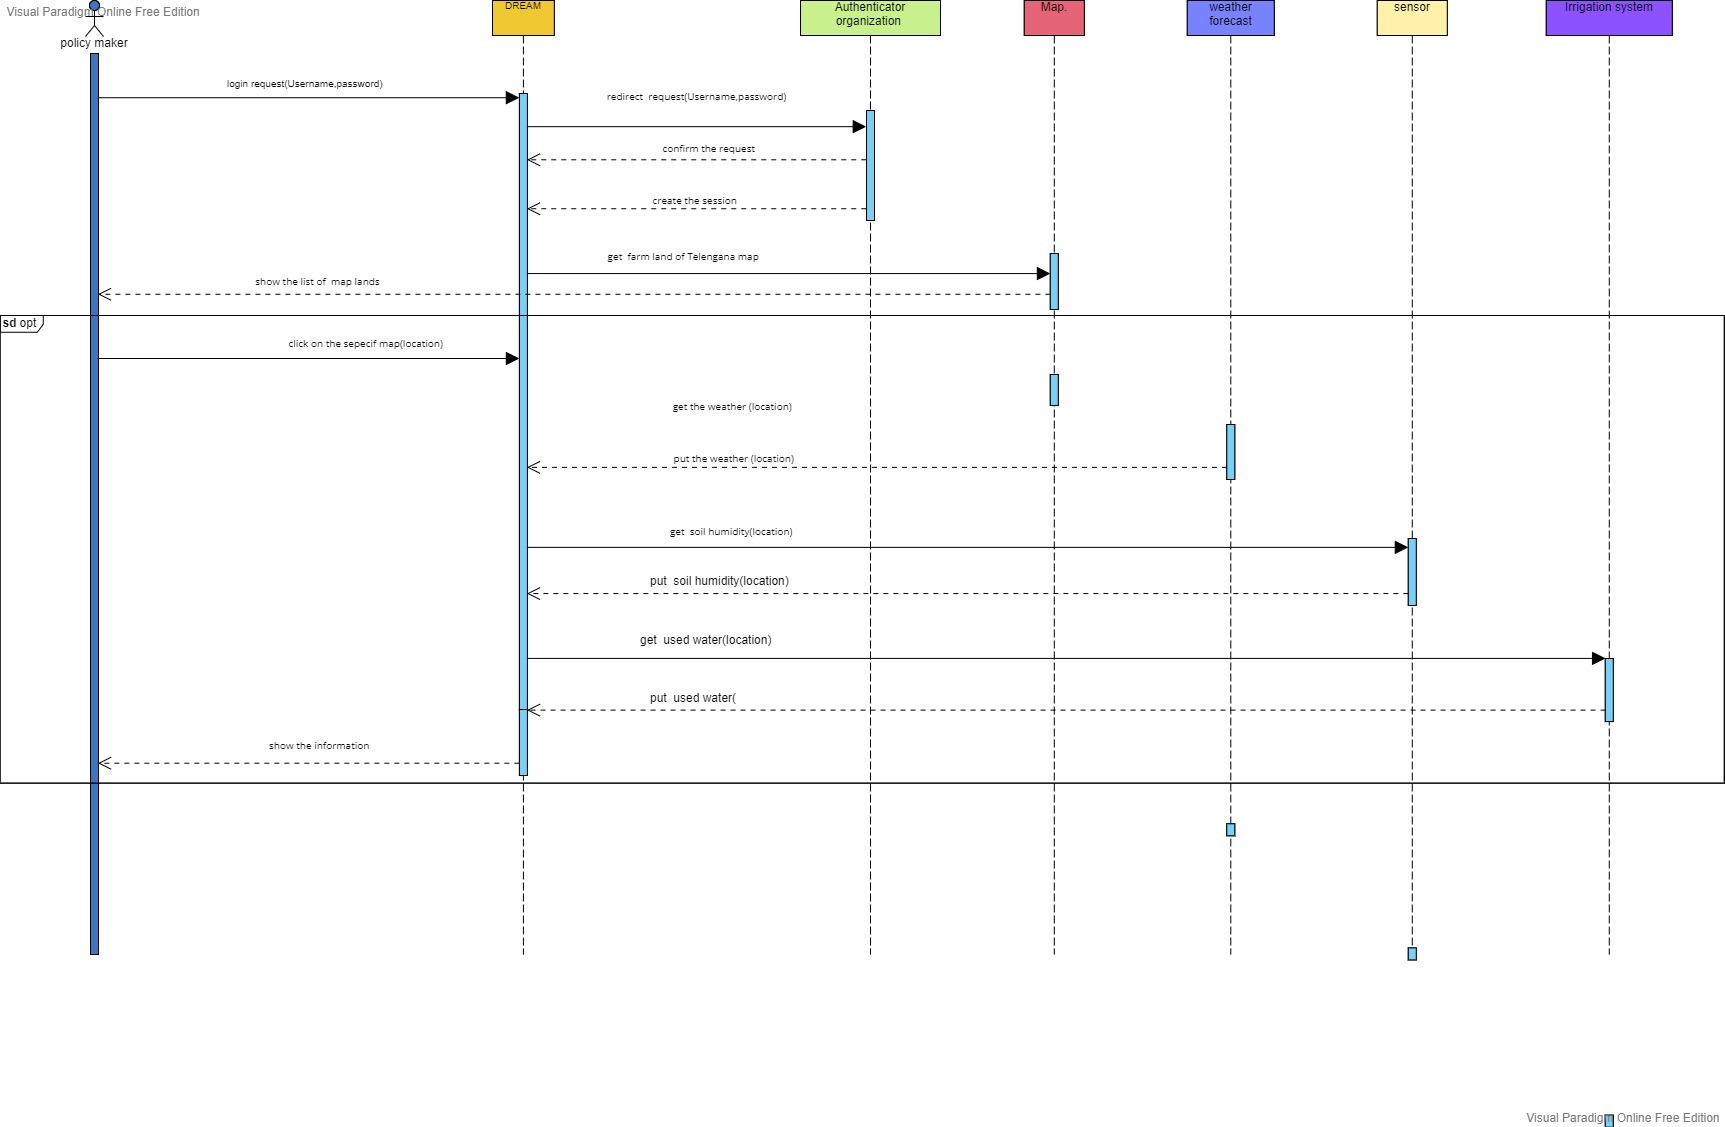
\includegraphics[width=1\textwidth]{figures/SecondSequenceDiagram.jpg}
%\caption{\label{fig:student } State Diagram 3 - evaluate the farmer by policymaker }
\end{figure}
\begin{figure}[H]
%\centering
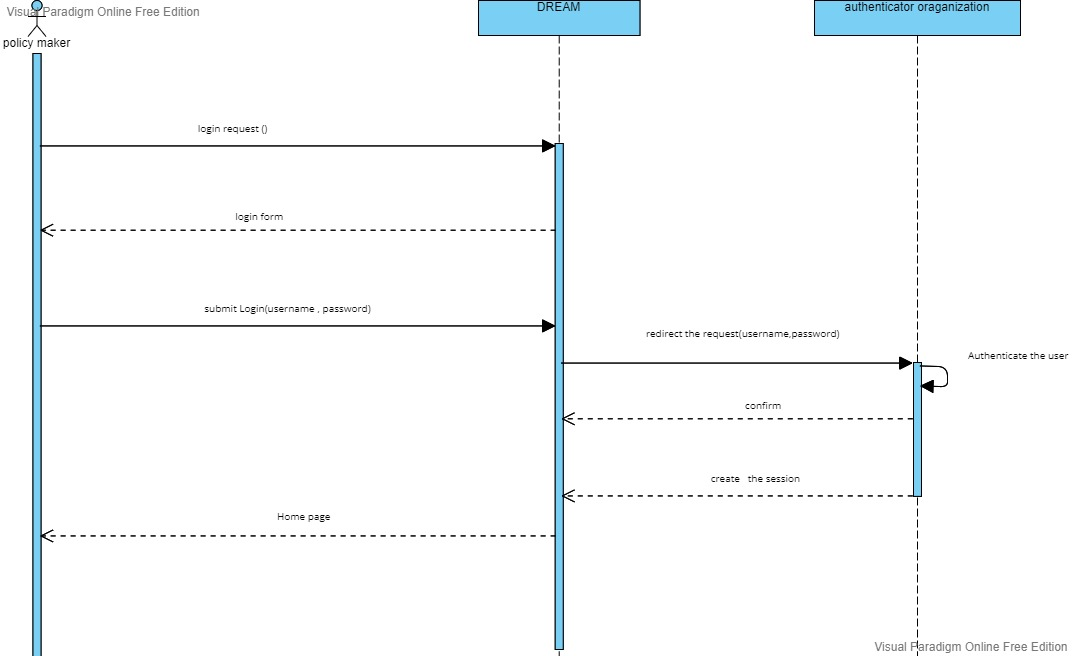
\includegraphics[width=1\textwidth]{figures/thirdSequenceDiagram.jpg}
%\caption{\label{fig:student } State Diagram 3 - evaluate the farmer by policymaker }
\end{figure}
\begin{figure}[H]
%\centering
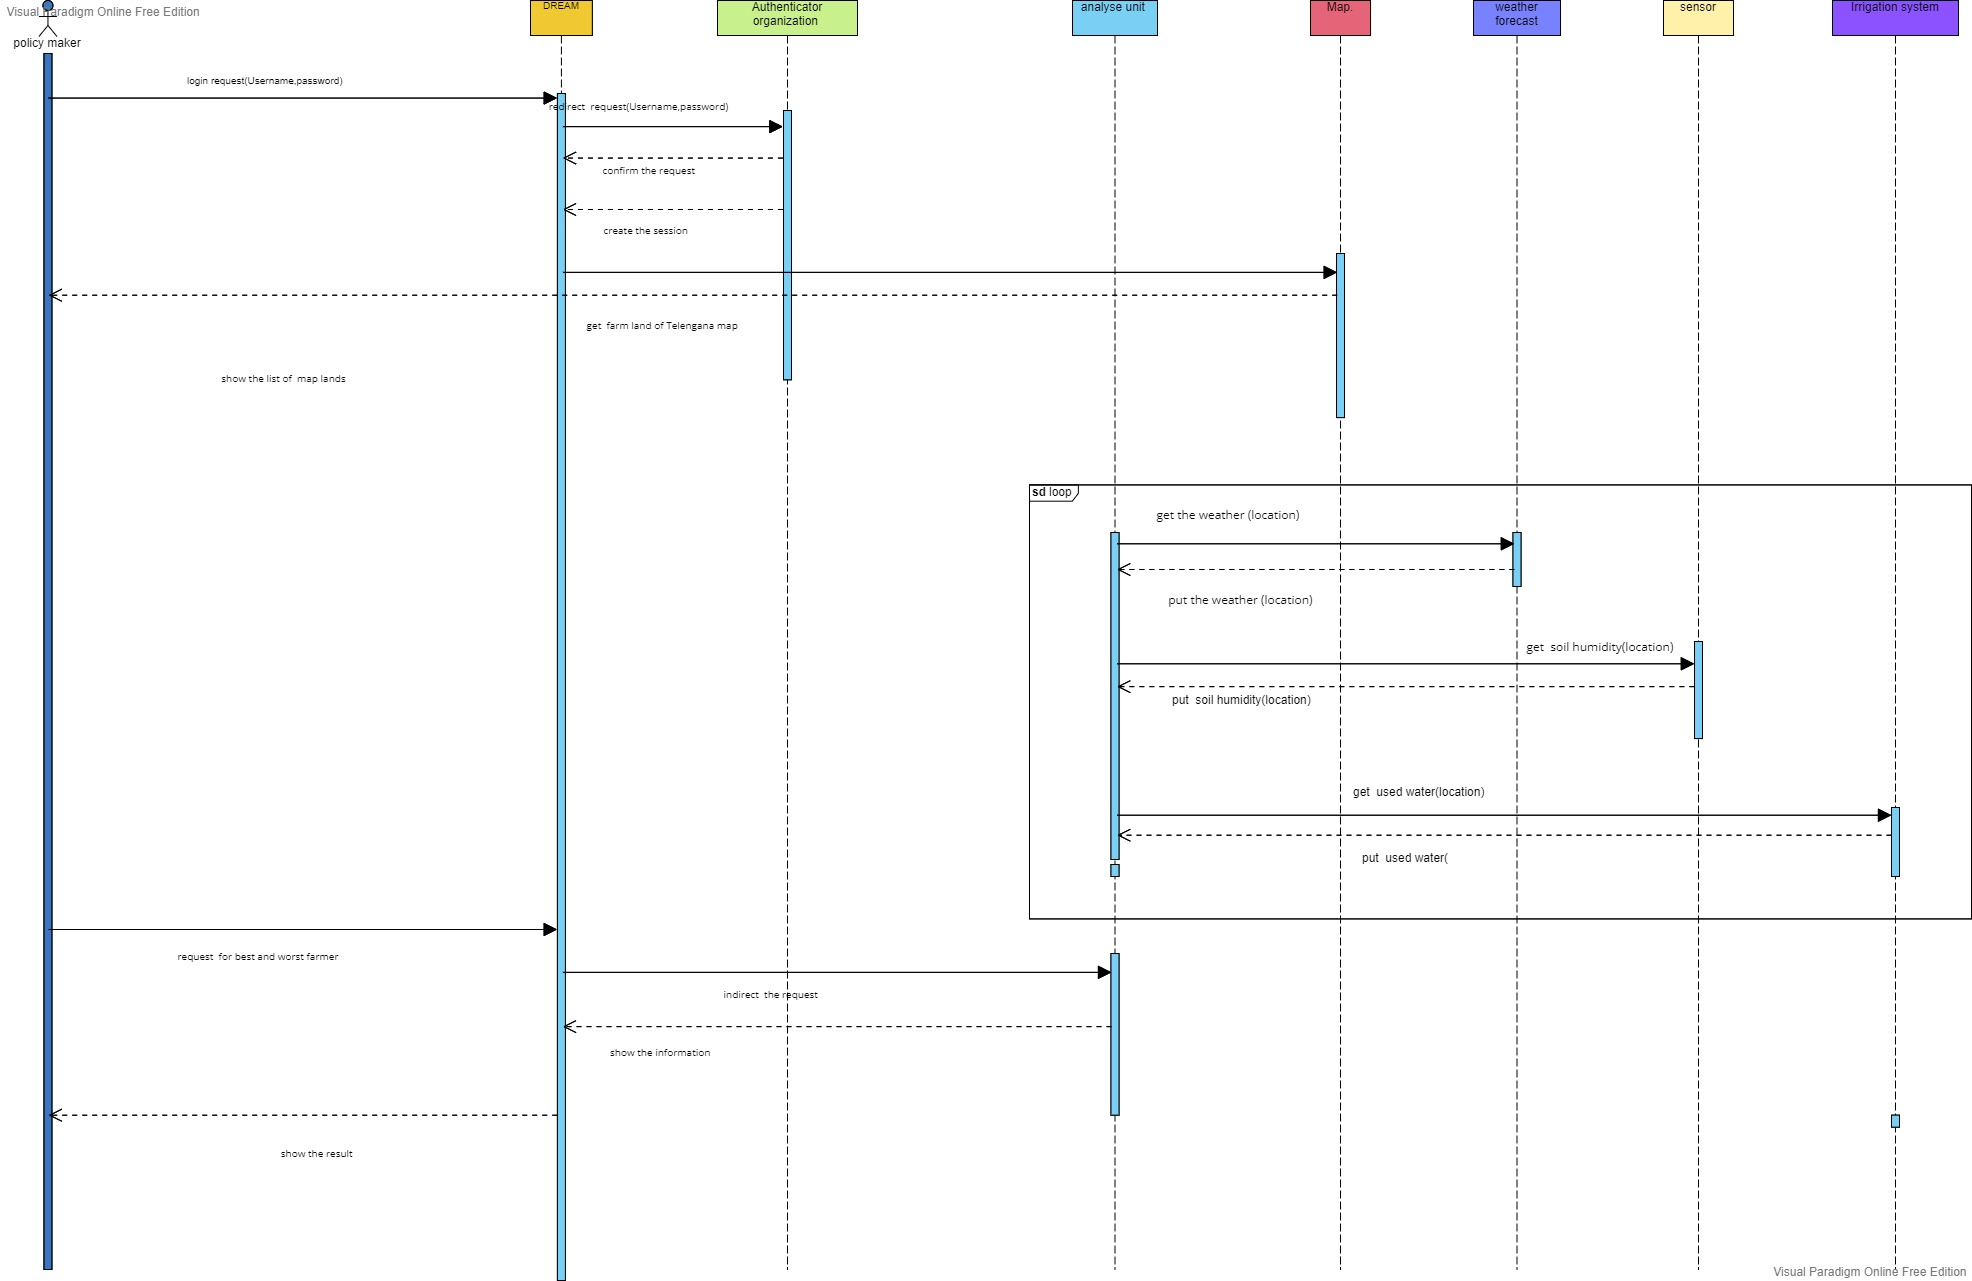
\includegraphics[width=1\textwidth]{figures/forthSequenceDiagram.jpg}
%\caption{\label{fig:student } State Diagram 3 - evaluate the farmer by policymaker }
\end{figure}

\begin{figure}[H]
%\centering
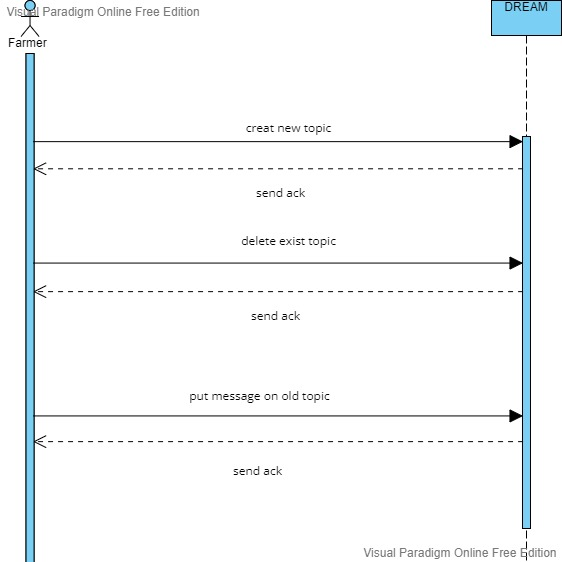
\includegraphics[width=1\textwidth]{figures/fifthSequenceDiagram.jpg}
%\caption{\label{fig:student } State Diagram 3 - evaluate the farmer by policymaker }
\end{figure}
\clearpage
    \subsubsection{Scenarios}
 \textbf{General}\\
    Nila is a farmer and as she was a teenager she start working on the land with her father. She starts working every day from 4:00 Am until 7:00 Pm on the land and check all the products qualities, the fertilizers, and the harvest time. So, she downloads this application, inserted the data of her land and the products, the beginning and ending time that she should implement or harvest the products and by using this app she can follow the progress of her land and see if there are some mismatches on the data that she got from the application and the products that she plants.
\newline
\\
\textbf{Ask for Assistant}\\
Aadhya is a middleman farmer who is tired of a new kind of pest last month. After he sold the product of his last harvest and calculated his benefit, he figured out it was negative, and he didn’t have any profit because his last products are attacked by the pests, and he had to pay lots of money to kill them and use more fertilizers to resuscitate the soil so he earn nothing. So, he downloads this application inserted the data of his land and by searching in the discussions he found some useful information from other farmers that had this problem and found a good solution to harness them. So he uses these devices and until now he gets a good result.
\newline
\\
\textbf{Be mechanized}\\
Tom is a farmer who used traditional farming. His son is going to start working with him and he wants to improve the quality of the product and increase their performance. As their land is too wide they need some help, for example, more workers or using some new technologies. He decided to insert some sensors in their land to be more mechanized. These sensors can measure the humidity of the soil and also by using the DREAM application they can insert the data about their products and also track the humidity of their soil and product. Also by using the data that we have from the weather forecast and personalizing suggestions, they decrease the amount of water that they need in irrigation or the number of fertilizers that they need. By using this approach Krishna’s son could increase their performance by about 10\% in just 2 months after using them and he hopes that they can increase the performance by about 20% in the next month.
\newline
\\
\textbf{faster comments}\\
Sarah is a policymaker in Telengana and she tracks the performance and quality of products for about 2 years. Now she figured out there was some aspect that she didn’t consider these years because of the number of farmers and different features that she had to track. Also, most of the comments that she sent for the farmers were useless because she couldn’t track their progress in real-time, and when she sent them because of changes that they had for example changing season most of them wasn’t useful anymore. She didn’t have any platform that shows the progress of a farmer or farmland for a period of time and she had to compare lots of paper things and it is obvious that she drop some points. After she started using DREAM she can observe the progress of farmers faster, send suggestions sooner so she got better results from her observation, and she saw the comments that she send for the farmers are more useful than before.
\newline
\\
\textbf{Best farmer}\\
Krishna one of the policymakers should evaluate the result of the farmers, she wants to know who has the best and worst approaches according to the information registered in the system, she logs in the application with official mail after the authentication, she goes to the rank section and sees the result.
\newline
\\
\textbf{Commenting}\\
Moila is an inexperienced farmer who wants to start farming on her land, she wants to use the experience of others to improve her knowledge so she decided to subscribe to the "how to get a crop from the land" and read the comments also she post her questions 

\newline
\subsection{Performance Requirements-Non-Functional Requirements}
The system should be able to guarantee a safe and consistent connection. Based on the population of Telangana in the worst case, the application should handle about 360,000 users that is the number of Telangana’s farmers. Also because most of the farmers work after the sunrise until the sunset so we must expect some burst in our requests. 
\subsection{Design Constraints - Non-Functional Requirements}
    \subsubsection{Standards compliance}
    The code should follow the requirements contained in this document. Furthermore, its comments should be clear and focused.
    \subsubsection{Hardware limitations}
    The software application requires a mobile device able to capture the position. In alternative, the authorities, can use a computer to observe the progress of the farmers. Both devices can be able to send data to the software via internet connection.
    \subsubsection{Any other constraint}
    The user has the limitation of being the owner of more than one farmland simultaneously.
\subsection{Software System Attributes - Non-Functional Requirements}
    \subsubsection{Reliability and availability}
    The application provides a reliable service in which individual farmers can easily log in and see the data related to their lands. Furthermore, it warranties that the chain of custody of the information coming from the farmers, sensors, and other systems is never broken, and the information is never altered. This would provide a secure and reliable system.
    
    The application must offer availability in the order of 99\% granting with at least 20 hours in a day. The lack of service must be minimal. It’s better to maintain system at nights and before the sunrise because farmers mostly do not use this application at night. Even at night, we could put some resources at sleep mode to reduce the cost of application.
    
    \subsubsection{Security}
    The users’ location and personal data is a very important data and must be encrypted so this part must be more secure than other data stores in the application. Moreover, in case of password recovery this should never be sent in clear. The system must be behind a proxy servers (like cloudflare) to prevent the DDoS attacks
    \subsubsection{Maintainability}
    The application must keep a service log in order to fix bugs more easily. The app should be developed using a micro-service approach, so adding new functions shouldn't’t require to change the previous code, and we can have different instance of services in different time of day. This application needs infrastructure like kubernetes to orchestrate the containers.
    \subsubsection{Portability}
    The user side must be available in different platform like Android, iOS and Web. The back-end side is better to be deployed with docker to easily deploy on any server.
    \subsubsection{Scalability}
    As Climate change continues to be a real and potent threat to the agriculture sector and food demand is expected to increase anywhere, so we will predict that so many farmers will join this app to track their progress, so the system must have a good infrastructure that could balance the loads and easily we must add new resources to it.
\subsection{Additional Specifications}
    \subsubsection{Mandatory Fields}
    At the moment of the registration, an authority will have to compile the following mandatory fields:
    \begin{itemize}
        \item Exact location of each farm land
        \item The products that each farmer has in his land
        \item Phone number
        \item Official Email for policymakers
    \end{itemize}
    %\subsubsection{Types of Violations}
    %\subsubsection{Types of Query}

    \clearpage


